%%%%%%%%%%%%%%%%%%%%% PACKAGE IMPORTS %%%%%%%%%%%%%%%%%%%%%
\documentclass{article}
\usepackage{import}
\subimport*{./}{macro}

\usepackage{amsmath, amsfonts, amsthm, amssymb}
\usepackage{lmodern}
\usepackage{microtype}
\usepackage{fullpage}       
\usepackage{changepage}
\usepackage{hyperref}
\usepackage{blindtext}
\usepackage{subcaption}
\hypersetup{
    colorlinks=true,
    linkcolor=blue,
    filecolor=magenta,      
    urlcolor=blue,
    pdftitle={Overleaf Example},
    pdfpagemode=FullScreen,
    }
\urlstyle{same}

\newenvironment{level}%
{\addtolength{\itemindent}{2em}}%
{\addtolength{\itemindent}{-2em}}

\usepackage{amsmath,amsthm,amssymb}

\usepackage[nooldvoltagedirection]{circuitikz}
\usetikzlibrary{decorations,arrows,shapes}

\usepackage{datetime}
\usepackage{etoolbox}
\usepackage{enumerate}
\usepackage{enumitem}
\usepackage{listings}
\usepackage{array}
\usepackage{varwidth}
\usepackage{tcolorbox}
\usepackage{amsmath}
\usepackage{circuitikz}
\usepackage{verbatim}
\usepackage[linguistics]{forest}
\usepackage{listings}
\usepackage{xcolor}
\renewcommand{\rmdefault}{cmss}


\newcommand\doubleplus{+\kern-1.3ex+\kern0.8ex}
\newcommand\mdoubleplus{\ensuremath{\mathbin{+\mkern-10mu+}}}

\definecolor{codegreen}{rgb}{0,0.6,0}
\definecolor{codegray}{rgb}{0.5,0.5,0.5}
\definecolor{codepurple}{rgb}{0.58,0,0.82}
\definecolor{backcolour}{rgb}{0.95,0.95,0.92}

\lstdefinestyle{mystyle}{
    language=Python,
    basicstyle=\ttfamily\small,
    keywordstyle=\color{blue},
    stringstyle=\color{red},
    commentstyle=\color{green},
    morecomment=[l][\color{magenta}]{\#},
    backgroundcolor=\color{backcolour},   
    breakatwhitespace=false,         
    breaklines=true,                 
    captionpos=b,                    
    keepspaces=true,                 
    numbers=left,                    
    numbersep=5pt,                  
    showspaces=false,                
    showstringspaces=false,
    showtabs=false,                  
    tabsize=2
}

\lstset{style=mystyle}
\setlength{\parindent}{0pt}
\setlength{\parskip}{5pt plus 1pt}

\providetoggle{questionnumbers}
\settoggle{questionnumbers}{true}
\newcommand{\noquestionnumbers}{
    \settoggle{questionnumbers}{false}
}

\newcounter{questionCounter}
\newenvironment{question}[2][\arabic{questionCounter}]{%
    \ifnum\value{questionCounter}=0 \else {\newpage}\fi%
    \setcounter{partCounter}{0}%
    \vspace{.25in} \hrule \vspace{0.5em}%
    \noindent{\bf \iftoggle{questionnumbers}{Question #1: }{}#2}%
    \addtocounter{questionCounter}{1}%
    \vspace{0.8em} \hrule \vspace{.10in}%
}

\newcounter{partCounter}[questionCounter]
\renewenvironment{part}[1][\alph{partCounter}]{%
    \addtocounter{partCounter}{1}%
    \vspace{.10in}%
    \begin{indented}%
       {\bf (#1)} %
}{\end{indented}}

\def\indented#1{\list{}{}\item[]}
\let\indented=\endlist
\def\show#1{\ifdefempty{#1}{}{#1\\}}
\def\IMP{\longrightarrow}
\def\AND{\wedge}
\def\OR{\vee}
\def\BI{\leftrightarrow}
\def\DIFF{\setminus}
\def\SUB{\subseteq}


\newcolumntype{C}{>{\centering\arraybackslash}m{1.5cm}}
\renewcommand\qedsymbol{$\blacksquare$}
\newtcolorbox{answer}
{
  colback   = green!5!white,    % Background colorucyitc,
  colframe  = green!75!black,   % Outline color
  box align = center,           % Align box on text line
  varwidth upper,               % Enables multi line input
  hbox                          % Bounds box to text width
}

\newcommand{\myhwname}{CSE 446 Homework 1}
\newcommand{\myname}{Sebastian Liu}
\newcommand{\myemail}{ll57@cs.washington.edu}
\newcommand{\mysection}{AB}
\newcommand{\dollararrow}{\stackrel{\$}{\leftarrow}}
%%%%%%%%%%%%%%%%%%%%%%%%%%%%%%%%%%%%%%%%%%%%%%%%%%%%%%%%%%%

%%%%%%%%%%%%%%%%%%% Document Options %%%%%%%%%%%%%%%%%%%%%%
\noquestionnumbers
%%%%%%%%%%%%%%%%%%%%%%%%%%%%%%%%%%%%%%%%%%%%%%%%%%%%%%%%%%%

%%%%%%%%%%%%%%%%%%%%%%%% WORK BELOW %%%%%%%%%%%%%%%%%%%%%%%%
\begin{document}

\begin{center}
    \textbf{Homework 1} \bigskip
\end{center}

%%%%%%%%%%%%%%%%%%%%%%%% Task 1 %%%%%%%%%%%%%%%%%%%%%%%%M
\begin{question}{A1.}
    \begin{part}
       \begin{answer}
            \textbf{Bias} is the difference between the expected value of our model and the true value we are trying to predict. When our model oversimplifies
            the "true distribution", we tend to have high bias.\\\\
            \textbf{Variance} describes the sensitivity of our model to data changes (i.e. how much our estimation will change as
            the data changes). When our model is overly complex (i.e. overfitting the data), we tend to have high variance.\\\\
            \textbf{Bias-variance tradeoff} is about finding the balance between bias and variance when modeling the distribution. We want to find the
            model that minimizes both bias and variance (i.e. the model that is not too simple or too complex), generalizing the trend, while keeping the
            necessary details to closely fit the data.
        \end{answer}
    \end{part}

    \begin{part}
        \begin{answer}
            \textbf{When model complexity increases,} its bias usually decreases while its variance tend to increase. \\\\
            \textbf{When model complexity decreases,} its bias usually increases while its variance tend to decrease. \\\\

            e.g. In the case of linear regression, when we increase the degree of the polynomial, we are increasing
            the complexity of the model. As a result, the model will be able to fit the data more closely, but it will also
            be more sensitive to changes in the data (more oscillation in the graph), which is equivalent of saying
            that the bias will decrease, while variance will increase. The opposite is true when we decrease the
            degree (complexity) of the polynomial.
         \end{answer}
     \end{part}

     \begin{part}
        \begin{answer}
            \textbf{False}. When we collect more data from the same distribution, the variance typically decreases.\\\\
            \textbf{Justification:}
            More data helps the model better understand the underlying "true distribution", reducing its sensitivity to small
            fluctuations in the training set (the noises get "averaged out"). Therefore, the prediction is more stable and
            the variance decreases.
         \end{answer}
     \end{part}
\newpage
     \begin{part}
        \begin{answer}
            \textbf{The validation set} should be used for hyperparameter tuning.\\\\
            If we use the training or the test set for hyperparameter tuning, the resulting model will be biased
            towards the specific training or test set. That's why validation exist in the first place (to minimizes
            the bias in hyperparameter tuning).\\\\
            \textbf{Let's take LOO as an example:} 
            \begin{itemize}
                \item Assume we have a dataset $D$ with a set of hyperparameters to tune.
                \item Let $D \setminus j$ be training data with $j$th data point $(x_j ,y_j)$ moved to validation set.
                \item We train the model $f_{D \setminus j}$ with $D \setminus j$ dataset.
                \item We estimate the true error of $f_{D \setminus j}$ on the predicting $y_j$ ($\{x_j, y_j\}$ is the
                validation set).
                \item We repeat the process for all $j$th data point in $D$ (for each data point we leave out we learn a
                $f_{D \setminus j}$).
                \item Average over all data points $j$ to get the LOO error.
                \item Repeat the process for all hyperparameters to get the LOO error for each hyperparameter.
                \item Pick the hyperparameter with the lowest LOO error.
                \item Train the model with the chosen hyperparameter on the entire dataset $D$.
                \item We test the model on the test set to get its performance on unseen data.
            \end{itemize}
        \end{answer}
     \end{part}

     \begin{part}
        \begin{answer}
            \textbf{False}. The training error of a function on the training set typically gives an underestimation of
            the true error.\\\\

            \textbf{Justification:} When we train a model on a training set, the model will learn the pattern from the specific
            dataset, which means that it should predict the training set pretty well (i.e. the training error will be low).
            However, the pattern in the specific training set, especially for small datasets, might not generalize well for
            unseen data. So, the model might not predict unseen data as well (i.e. the true error might be higher).
            Therefore, the training error should be an underestimation of the true error.
        \end{answer}
     \end{part}
\end{question}

%%%%%%%%%%%%%%%%%%%%%%%% Task 2 %%%%%%%%%%%%%%%%%%%%%%%%
\begin{question}{A2.}
    \begin{part}
        \begin{answer}
            \begin{align*}
                \widehat{\lambda}_\text{MLE} &= \underset{\lambda}{\argmax} \Prob{x \mid \lambda} \\
                &= \underset{\lambda}{\argmax} \;\; \log \Prob{x \mid \lambda}\\
                &= \underset{\lambda}{\argmax} \;\; \log \prod_{i=1}^n \Prob{x_i \mid \lambda} \\
                &= \underset{\lambda}{\argmax} \;\; \sum_{i=1}^n \log \Prob{x_i \mid \lambda} \\
                &= \underset{\lambda}{\argmax} \;\; \sum_{i=1}^n \log e^{-\lambda} \frac{\lambda^x_i}{x_i!} \\
                &= \underset{\lambda}{\argmax} \;\; \sum_{i=1}^n \log e^{-\lambda} +
                \log \lambda^x_i - \log x_i! \\
                &= \underset{\lambda}{\argmax} \;\; \sum_{i=1}^n -\lambda +
                x_i \log \lambda - \log x_i! \\
                &\Rightarrow \deriv{}{\lambda} \sum_{i=1}^n -\lambda +
                x_i \log \lambda - \log x_i! = 0 \tag{set derivative to 0} \\
                &\Rightarrow \sum_{i=1}^n -1 + \frac{x_i}{\lambda} = 0 \\
                &\Rightarrow \sum_{i=1}^n \frac{x_i}{\lambda} = \sum_{i=1}^n 1 \\
                &\Rightarrow \boxed{\widehat{\lambda}_\text{MLE} = \frac{1}{n} \sum_{i=1}^n x_i}
           \end{align*}
         \end{answer}
     \end{part}

     \begin{part}
        \begin{answer}
            \begin{align*}
                \widehat{\lambda}_\text{MLE} &= \frac{1}{n} \sum_{i=1}^n x_i \tag{from part (a)} \\
                &= \frac{1}{5} (3 + 7 + 5 + 0 + 2) \tag{plug in the first 5 data points} \\
                &= \boxed{3.4}
            \end{align*}
            $$\text{Poi} (x = 4 \mid \lambda = 3.4) = \boxed{e^{-3.4} \cdot \frac{3.4^4}{4!} \approx 0.1858 }$$
         \end{answer}
     \end{part}
\newpage
     \begin{part}
        \begin{answer}
            \begin{align*}
                \widehat{\lambda}_\text{MLE} &= \frac{1}{n} \sum_{i=1}^n x_i \tag{from part (a)} \\
                &= \frac{1}{6} (3 + 7 + 5 + 0 + 2 + 8) \tag{plug in the first 6 data points} \\
                &= \boxed{\frac{25}{6}}
            \end{align*}
            $$\text{Poi} (x = 5 \mid \lambda = \frac{25}{6}) = \boxed{e^{-\frac{25}{6}} \cdot \frac{(\frac{25}{6})^5}{5!} \approx 0.1623 }$$
        \end{answer}
     \end{part}

\end{question}

%%%%%%%%%%%%%%%%%%%%%%%% Task 3 %%%%%%%%%%%%%%%%%%%%%%%%
\begin{question}{A3. } 
     \begin{part}[b]
        \begin{figure}[h]
            \centering
            \begin{subfigure}{.49\textwidth}
              \centering
              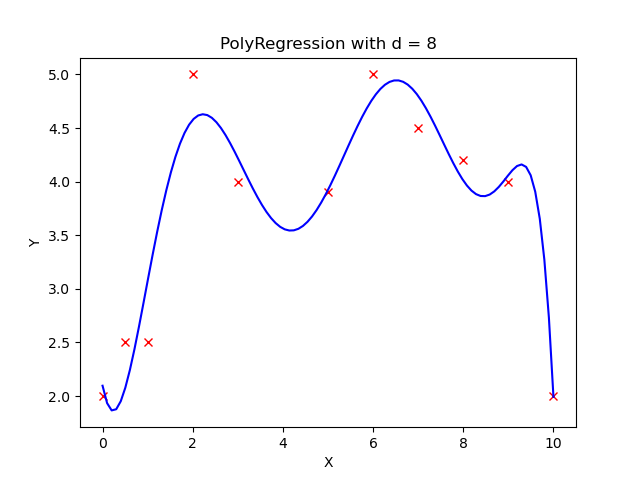
\includegraphics[width=\linewidth]{./img/lam0.png}
              \caption{$\lambda = 0$}
            \end{subfigure}
            \begin{subfigure}{.49\textwidth}
              \centering
              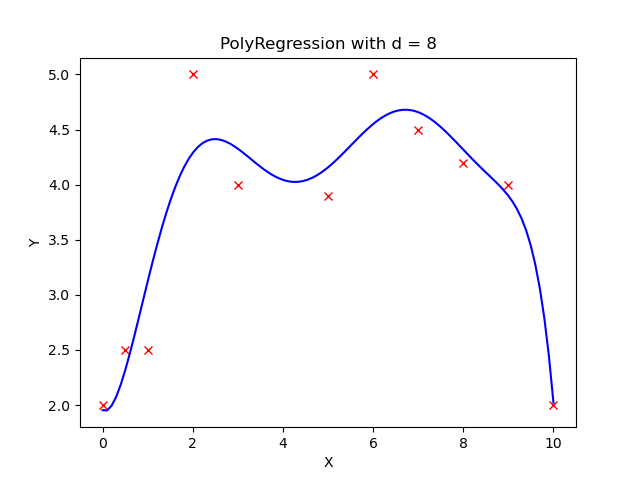
\includegraphics[width=\linewidth]{./img/lam1e-7.png}
              \caption{$\lambda = 1e-7$}
            \end{subfigure}
            \begin{subfigure}{.49\textwidth}
                \centering
                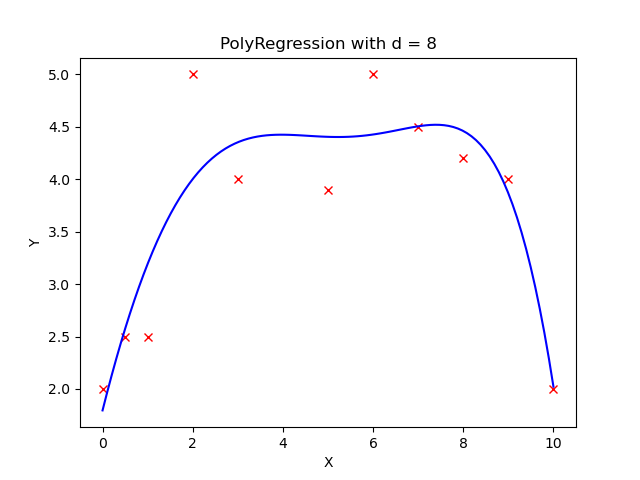
\includegraphics[width=\linewidth]{./img/lam1e-4.png}
                \caption{$\lambda = 1e-4$}
            \end{subfigure}
            \begin{subfigure}{.49\textwidth}
                \centering
                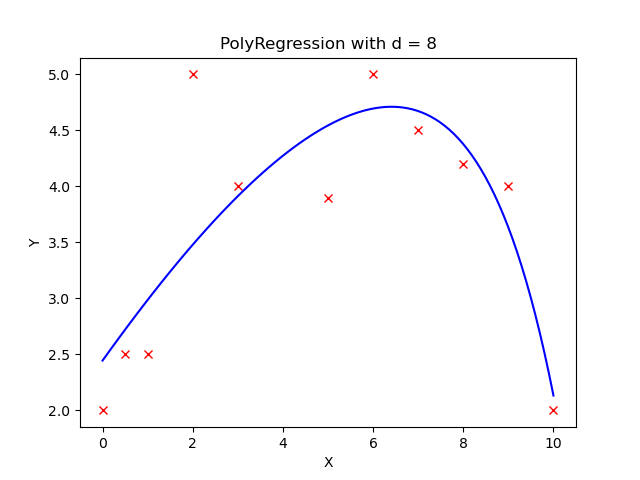
\includegraphics[width=\linewidth]{./img/lam1e-1.png}
                \caption{$\lambda = 1e-1$}
            \end{subfigure}
            \end{figure}
            \begin{answer}
                As shown above, as regularization parameter $\lambda$ increases (from 0 to 0.1), the model puts more penalty on large weights which decreases variance.
                It resulted in smoother and less complex curves, which indicates that the model generalize better to new data points but has higher bias at the same time.
            \end{answer}
     \end{part}
\end{question}

%%%%%%%%%%%%%%%%%%%%%%%% Task 4 %%%%%%%%%%%%%%%%%%%%%%%%
\begin{question}{A4.}
        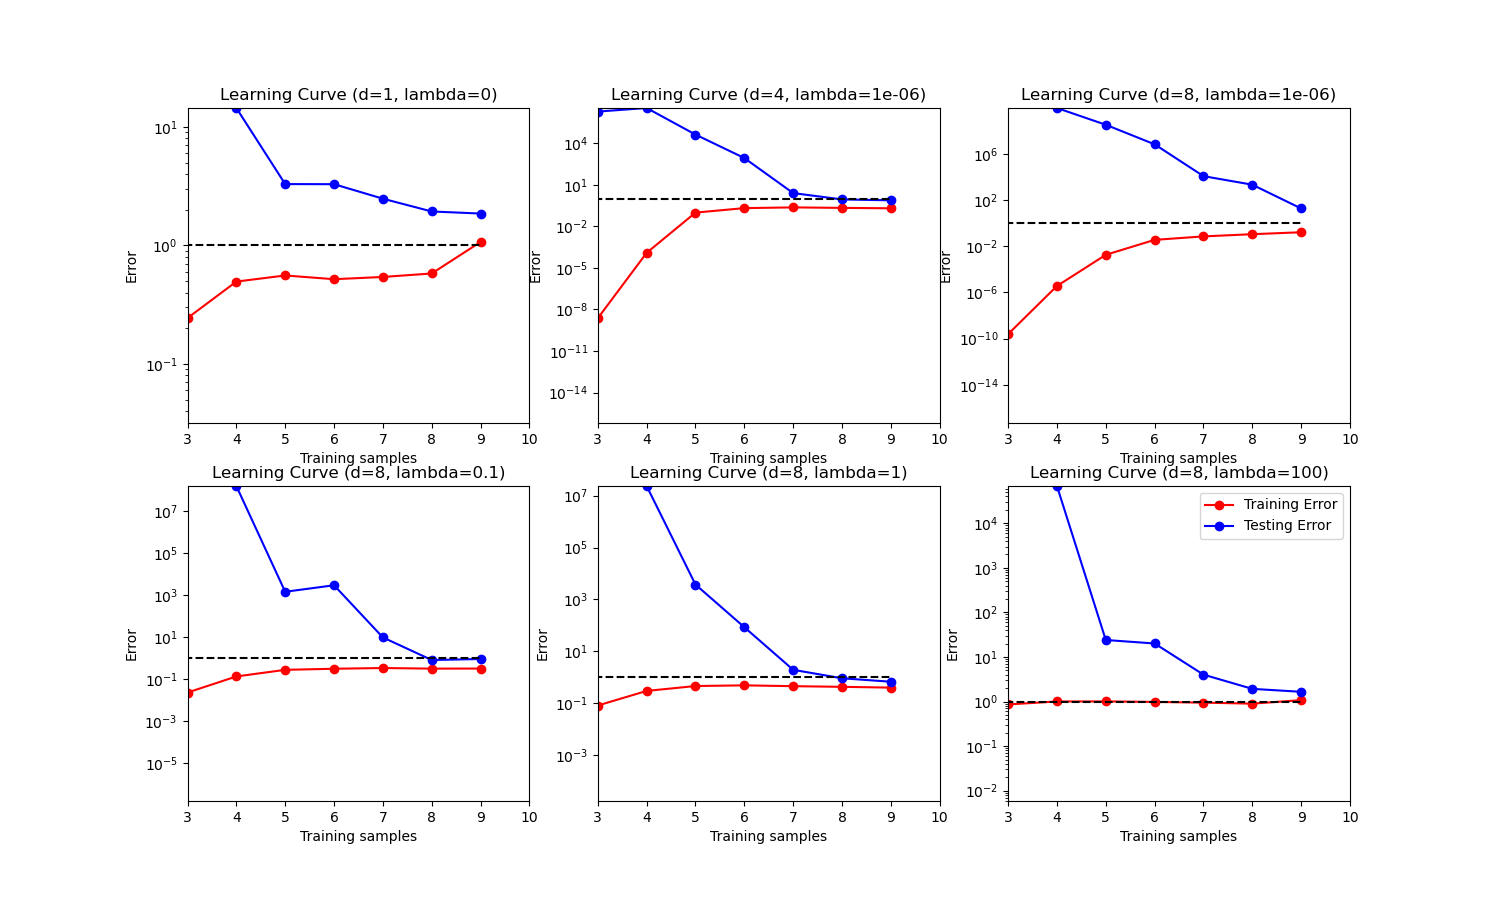
\includegraphics[width=1.2\linewidth]{./img/bias-variance.png}
\end{question}

%%%%%%%%%%%%%%%%%%%%%%%% Task 5 %%%%%%%%%%%%%%%%%%%%%%%%
\begin{question}{A5.} 
    \begin{part}
        \begin{answer}
            \begin{align*}
                \widehat{W} &= \underset{W}{\text{argmin}} \sum_{i=1}^{n} \| W^\top x_{i} - y_{i} \|^{2}_{2} + \lambda \|W\|_{F}^{2} \\
                &= \underset{W}{\text{argmin}} \sum_{j=1}^k \left[  \sum_{i=1}^n ( e_j^\top  W^\top  x_i - e_j^\top  y_i)^2 + \lambda \| W e_j \|^2_2 \right] \tag{$\arg\max_{j=0,\dots,9} e_{j+1}^\top  \widehat{W}^\top  x_i$ and $W = \begin{bmatrix} w_1 & \dots & w_k \end{bmatrix}$} \\
                &= \underset{W}{\text{argmin}} \sum_{j=1}^k \left[  \sum_{i=1}^n ( w_j^\top  x_i - e_j^\top  y_i)^2 + \lambda \| w_j \|^2_2 \right] \\
                &= \underset{W}{\text{argmin}} \sum_{j=1}^k \left[  \| X w_j - Y e_j\|^2_2 + \lambda \| w_j \|^2_2 \right] \tag{ Where $X = \begin{bmatrix} x_1 & \dots & x_n \end{bmatrix}^\top \in \R^{n \times d}$ and $Y = \begin{bmatrix} y_1 & \dots & y_n \end{bmatrix}^\top \in \R^{n \times k}$} \\
                &= \underset{W}{\text{argmin}} \sum_{j=1}^k \left[  (Xw_j - Ye_j)^\top (Xw_j - Ye_j) + \lambda w_j^\top  w_j  \right] \\
                &= \underset{W}{\text{argmin}} \sum_{j=1}^k \left[  (Xw_j)^\top  Xw_j - (Xw_j)^\top  Ye_j - (Ye_j)^\top  Xw_j + (Ye_j)^\top  Ye_j + \lambda w_j^\top  w_j  \right] \\
                &= \underset{W}{\text{argmin}} \sum_{j=1}^k  \left[  w_j^\top  X^\top  Xw_j - 2w_j^\top  X^\top   Ye_j + e_j^\top Y^\top  Ye_j + \lambda w_j^\top  w_j  \right] \\
                &= \underset{W}{\text{argmin}} \sum_{j=1}^k \left[  w_j^\top  (X^\top  X + \lambda I )w_j - 2w_j^\top  X^\top   Ye_j + e_j^\top Y^\top  Ye_j \right]
            \end{align*}
            We take gradient w.r.t $w_j$:
            \begin{align*}
                &\nabla_{w_j} \sum_{j=1}^k  \left[  w_j^\top  (X^\top  X + \lambda I )w_j - 2w_j^\top  X^\top   Ye_j + e_j^\top Y^\top  Ye_j \right]\\
                = &\sum_{j=1}^k \nabla_{w_j}(w_j^\top  (X^\top  X + \lambda I )w_j) - 2\nabla_{w_j}(w_j^\top  X^\top   Ye_j) + \nabla_{w_j}(e_j^\top Y^\top  Ye_j) \\
                = &\sum_{j=1}^k  2(X^\top  X + \lambda I )w_j - 2X^\top   Ye_j \tag{Since $X^\top  X + \lambda I$ is symmetric} \\
                = &2(X^\top  X + \lambda I )\sum_{j=1}^k w_j - 2X^\top  Y \sum_{j=1}^k e_j \\
                = &2(X^\top X + \lambda I)W - 2X^\top Y I \\ = &2(X^\top X + \lambda I)W - 2X^\top Y
            \end{align*}
            \end{answer}
        \end{part}
        \newpage
        \begin{part}[a contd.]
        \begin{answer}
            Setting the gradient to zero, we get:
            \begin{align*}
                & 2(X^\top  X + \lambda I ) \widehat{W} - 2X^\top Y = 0 \\
                &\Rightarrow (X^\top  X + \lambda I ) \widehat{W} = X^\top Y \\
                & \Rightarrow \boxed{\widehat{W} = (X^\top  X + \lambda I )^{-1} X^\top Y}
            \end{align*}
        \end{answer}
     \end{part}

     \begin{part}
        \begin{answer}
           \textbf{Training Error:} 14.805\% \\
           \textbf{Test Error:}  14.66\%
        \end{answer}
     \end{part}
     \newpage
     \begin{part}
        \begin{figure}[h]
            \centering
            \begin{subfigure}{.25\textwidth}
              \centering
              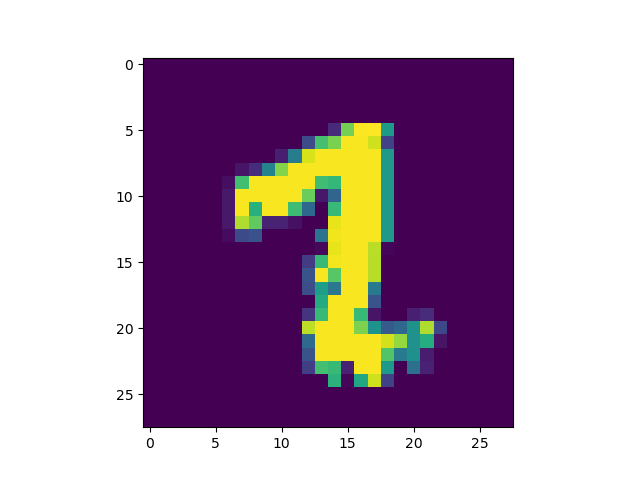
\includegraphics[width=\linewidth]{./img/2-1.png}
              \caption{$y = 2, \widehat{y} = 1$}
            \end{subfigure}
            \begin{subfigure}{.25\textwidth}
              \centering
              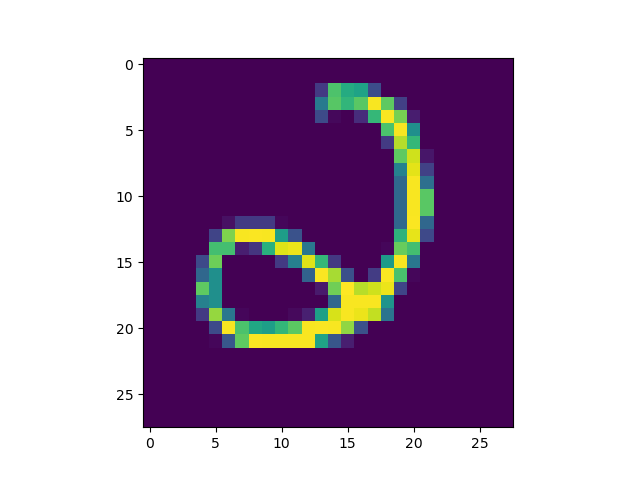
\includegraphics[width=\linewidth]{./img/2-6.png}
              \caption{$y = 2, \widehat{y} = 6$}
            \end{subfigure}
            \begin{subfigure}{.25\textwidth}
                \centering
                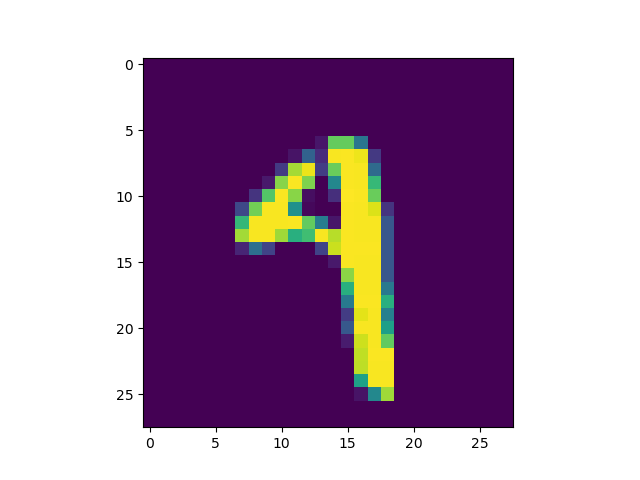
\includegraphics[width=\linewidth]{./img/4-9.png}
                \caption{$y = 4, \widehat{y} = 9$}
            \end{subfigure}
           \begin{subfigure}{.25\textwidth}
                \centering
                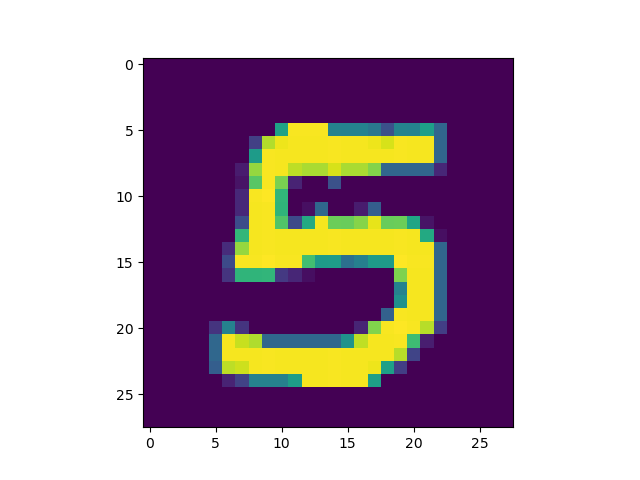
\includegraphics[width=\linewidth]{./img/5-3.png}
                \caption{$y = 5, \widehat{y} = 3$}
            \end{subfigure}
            \begin{subfigure}{.25\textwidth}
                \centering
                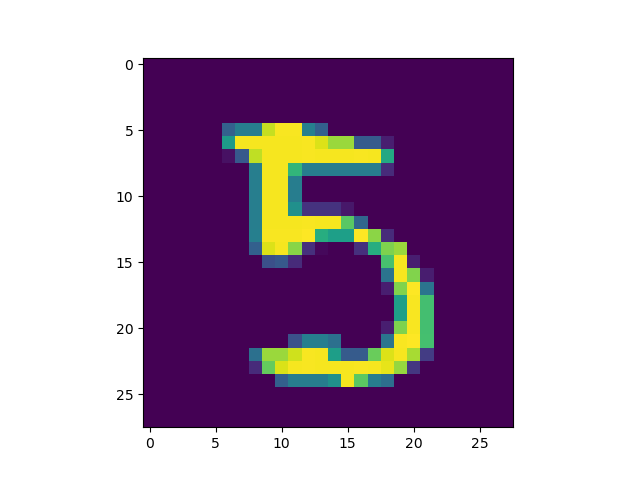
\includegraphics[width=\linewidth]{./img/5-3_.png}
                \caption{$y = 5, \widehat{y} = 3$}
              \end{subfigure}
              \begin{subfigure}{.25\textwidth}
                \centering
                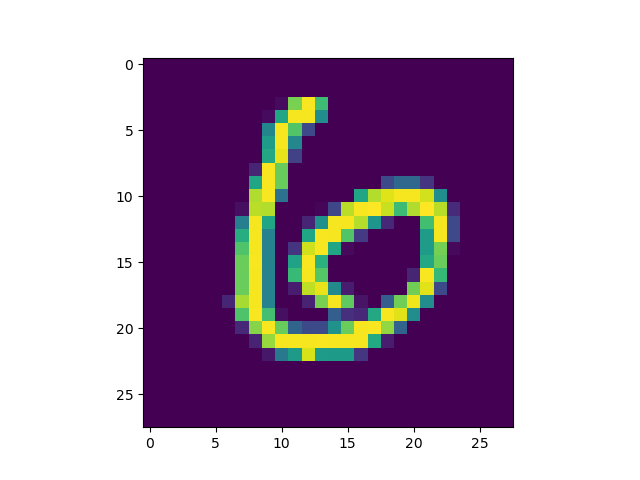
\includegraphics[width=\linewidth]{./img/6-4.png}
                \caption{$y = 6, \widehat{y} = 4$}
              \end{subfigure}
              \begin{subfigure}{.25\textwidth}
                  \centering
                  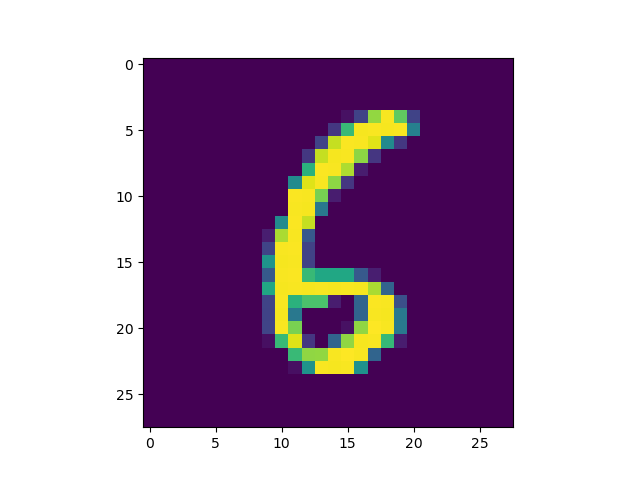
\includegraphics[width=\linewidth]{./img/6-8.png}
                  \caption{$y = 6, \widehat{y} = 8$}
              \end{subfigure}
              \begin{subfigure}{.25\textwidth}
                  \centering
                  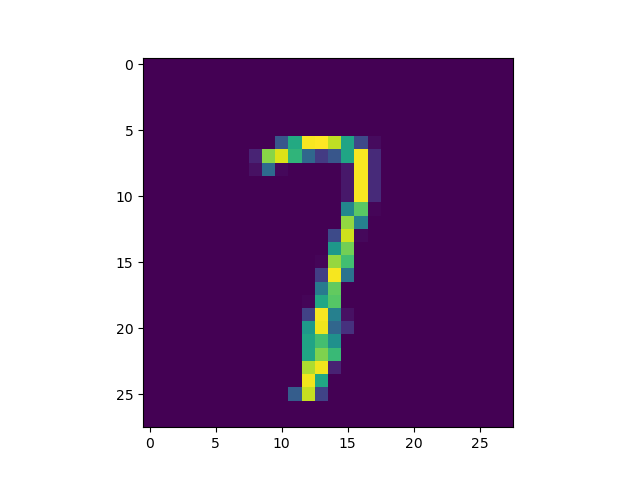
\includegraphics[width=\linewidth]{./img/7-1.png}
                  \caption{$y = 7, \widehat{y} = 1$}
              \end{subfigure}
              \begin{subfigure}{.25\textwidth}
                \centering
                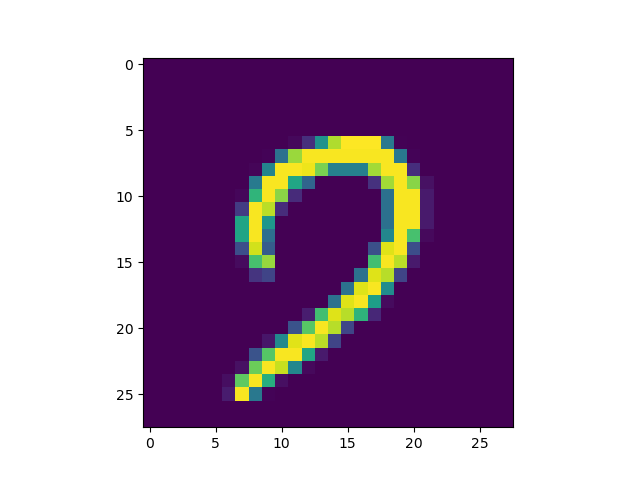
\includegraphics[width=\linewidth]{./img/7-9.png}
                \caption{$y = 7, \widehat{y} = 9$}
            \end{subfigure}
            \begin{subfigure}{.25\textwidth}
                \centering
                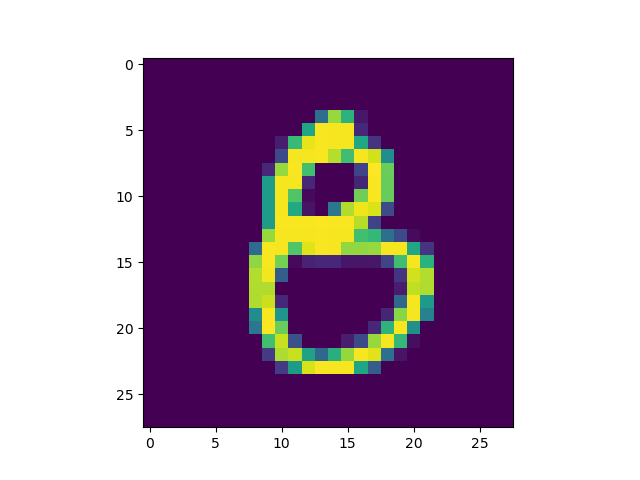
\includegraphics[width=\linewidth]{./img/8-3.png}
                \caption{$y = 8, \widehat{y} = 3$}
            \end{subfigure}
            \begin{subfigure}{.25\textwidth}
                \centering
                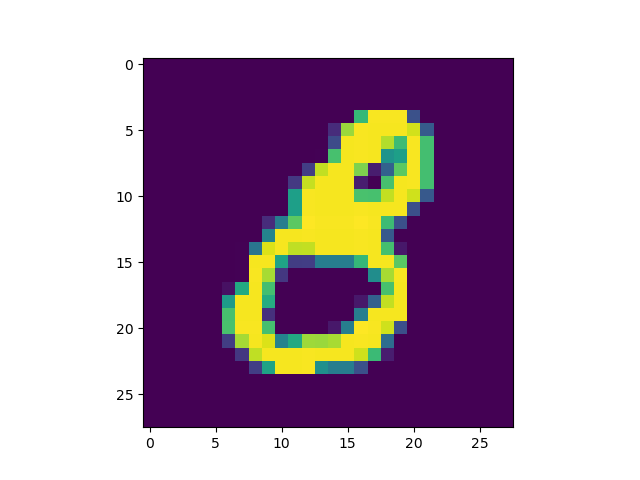
\includegraphics[width=\linewidth]{./img/8-3_.png}
                \caption{$y = 8, \widehat{y} = 3$}
            \end{subfigure}
            \begin{subfigure}{.25\textwidth}
              \centering
              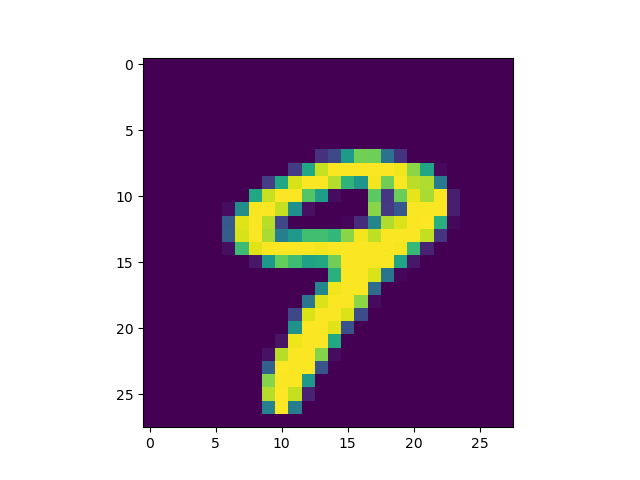
\includegraphics[width=\linewidth]{./img/9-7.png}
              \caption{$y = 9, \widehat{y} = 7$}
          \end{subfigure}
            \end{figure}
            \begin{answer}
                It seems that the classifier tends to confuse digits with similar
                structural features (similar shapes and strokes) or those that are poorly written.\\
                 Digits like 1 and 7, 1 and 2, 4 and 9 can be easily mixed up
                if the handwriting is ambiguous (true even for human).\\
                However, for digits that are structurally similar like 5 and 3, 8 and 3, the handwriting are
                pretty clear for human to distinguish, but the classifier still having a hard time
                telling them apart.\\
            \end{answer}
        \end{part}
    

\end{question}

%%%%%%%%%%%%%%%%%%%%%%%% Task 6 %%%%%%%%%%%%%%%%%%%%%%%%
\begin{question}{A6.} 
    \begin{part}
        \begin{answer}
            15 hours
         \end{answer}
     \end{part}

\end{question}
\end{document}
